\newpage
\section{Details of Pre-Training Experiment}


\subsection{Architecture and Hyperparameters}
We introduce details of the LLaMA architecture and hyperparameters used for pre-training. 
Table~\ref{tab:llama_hyperparameters} shows the most hyperparameters of LLaMA models across model sizes. 
We use a max sequence length of 256 for all models, with a batch size of 131K tokens.
For all experiments, we adopt learning rate warmup for the first 10\% of the training steps, and use cosine annealing for the learning rate schedule, decaying to 10\% of the initial learning rate.


\begin{table*}[h]
    \caption{Hyperparameters of LLaMA models for evaluation. Data amount are specified in tokens.}
    \label{tab:llama_hyperparameters}
    \vskip 0.15in
    \begin{center}
    \begin{tabular}{cccccccc}
    \toprule
    Params & Hidden & Intermediate & Heads & Layers & Steps & Data amount \\
    \midrule
    60M & 512 & 1376 & 8 & 8  & 10K & $1.3 \mathrm{~B}$ \\
    130M & 768 & 2048 & 12 & 12  & 20K & $2.6 \mathrm{~B}$ \\
    350M & 1024 & 2736 & 16 & 24  & 60K & $7.8 \mathrm{~B}$ \\
    $1 \mathrm{~B}$ & 2048 & 5461 & 24 & 32 & 100K & $13.1 \mathrm{~B}$ \\
    $7 \mathrm{~B}$ & 4096 & 11008 & 32 & 32 & 150K & $19.7 \mathrm{~B}$ \\
    \bottomrule
    \end{tabular}
    \end{center}
    \vskip -0.1in
\end{table*}

For all methods on each size of models (from 60M to 1B), we tune their favorite learning rate from a set of $\{0.01, 0.005, 0.001, 0.0005, 0.0001\}$, and the best learning rate is chosen based on the validation perplexity.
We find \lowrank{} is insensitive to hyperparameters and tends to be stable with the same learning rate across different model sizes.
For all models, \lowrank{} use the same hyperparameters, including the learning rate of $0.01$, scale factor $\alpha$ of $0.25$, and the subspace change frequency of $T$ of $200$. We note that since $\alpha$ can be viewed as a fractional learning rate, most of the modules (e.g., multi-head attention and feed-forward layers) in LLaMA models have the actual learning rate of $0.0025$.
This is, still, a relatively large stable learning rate compared to the full-rank baseline, which usually uses a learning rate $\leq 0.001$ to avoid spikes in the training loss.




\subsection{Memory Estimates}
As the GPU memory usage for a specific component is hard to measure directly, we estimate the memory usage of the weight parameters and optimizer states for each method on different model sizes.
The estimation is based on the number of original parameters and the number of low-rank parameters, trained by BF16 format.
For example, for a 60M model, LoRA ($r=128$) requires $42.7$M parameters on low-rank adaptors and $60M$ parameters on the original weights, resulting in a memory cost of $0.20$G for weight parameters and $0.17$G for optimizer states.
Table~\ref{tab:memory_estimate} shows the memory estimates for weight parameters and optimizer states for different methods on different model sizes, as a compliment to the total memory reported in the main text.

\begin{table*}[h]
    \caption{Memory estimates for weight parameters and optimizer states.}
    \label{tab:memory_estimate}
    \begin{subtable}{.5\linewidth}
        \centering
        \caption{Memory estimate of weight parameters.}
        \begin{tabular}{lcccc}
        \toprule
                   & \textbf{60M} & \textbf{130M} & \textbf{350M} & \textbf{1B} \\
        \midrule
        Full-Rank & 0.12G & 0.25G & 0.68G & 2.60G \\
        \midrule
        \textbf{\lowrank{}} & 0.12G & 0.25G & 0.68G & 2.60G \\
        Low-Rank & 0.08G & 0.18G & 0.36G & 1.19G \\
        LoRA & 0.20G & 0.44G & 1.04G & 3.79G \\
        ReLoRA & 0.20G & 0.44G & 1.04G & 3.79G \\
        \bottomrule
        \end{tabular}
    \end{subtable}%
    \begin{subtable}{.5\linewidth}
        \centering
        \caption{Memory estimate of optimizer states.}
        \begin{tabular}{lcccc}
        \toprule
                   & \textbf{60M} & \textbf{130M} & \textbf{350M} & \textbf{1B} \\
        \midrule
        Full-Rank & 0.23G & 0.51G & 1.37G & 5.20G \\
        \midrule
        \textbf{\lowrank{}} & 0.13G & 0.28G & 0.54G & 1.78G \\
        Low-Rank & 0.17G & 0.37G & 0.72G & 2.38G \\
        LoRA & 0.17G & 0.37G & 0.72G & 2.38G \\
        ReLoRA & 0.17G & 0.37G & 0.72G & 2.38G \\
        \bottomrule
        \end{tabular}
    \end{subtable}
\end{table*}

\newpage
\subsection{Training Progression}
We show the training progression of 130M, 350M, 1B and 7B models in Figure~\ref{fig:loss_curves}.
Compared to LoRA, GaLore closely matches the training trajectory of the full-rank baseline, and it even converges slightly faster at the beginning of the training. 

\begin{figure*}[h]
    \centering
    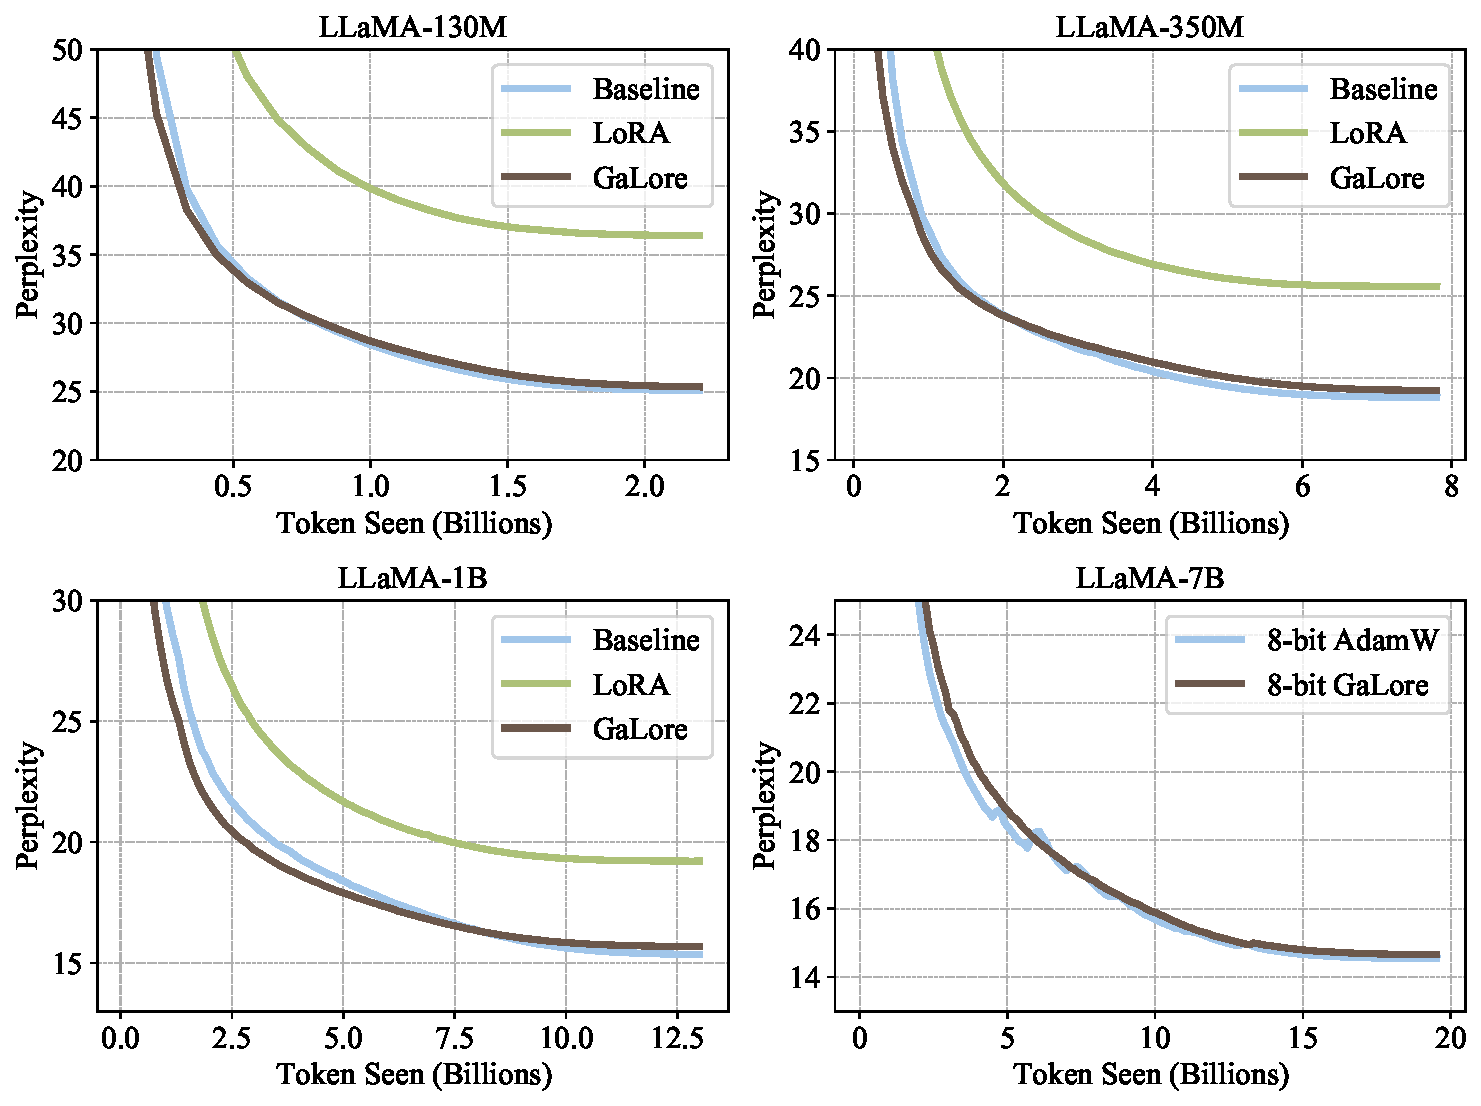
\includegraphics[width=0.8\textwidth]{figures/files/loss_curves.pdf}
    \caption{Training progression for pre-training LLaMA models on C4 dataset.}
    \label{fig:loss_curves}
\end{figure*}

\newpage
\section{Fine-Tuning Experiments}

\subsection{Details of Fine-Tuning on GLUE}

We fine-tune the pre-trained RoBERTa-Base model on the GLUE benchmark using the model provided by the Hugging Face\footnote{\url{https://huggingface.co/transformers/model_doc/roberta.html}}.
We trained the model for 30 epochs with a batch size of 16 for all tasks except for CoLA, which uses a batch size of 32.
We tune the learning rate and scale factor for \lowrank{}.
Table~\ref{tab:ft_hyperparameters} shows the hyperparameters used for fine-tuning RoBERTa-Base for \lowrank{}.


\begin{table*}[h]
    \caption{Hyperparameters of fine-tuning RoBERTa base for \lowrank.}
    \centering
    \label{tab:ft_hyperparameters}
    \begin{tabular}{ccccccccc}
    \toprule
    & MNLI   & SST-2 & MRPC    & CoLA    & QNLI    & QQP     & RTE     & STS-B   \\
    \midrule
    Batch Size    & 16     & 16    & 16      & 32      & 16      & 16      & 16      & 16      \\
    \# Epochs     & 30     & 30    & 30      & 30      & 30      & 30      & 30      & 30      \\
    Learning Rate & 1E-05  & 1E-05     & 3E-05   & 3E-05   & 1E-05   & 1E-05   & 1E-05   & 1E-05   \\    
    Rank Config. & & & & $r=4$ & & & & \\
    \lowrank \(\alpha\) & & & & 4 & & & & \\
    Max Seq. Len. & & & & 512 & & & & \\
    \bottomrule
    \end{tabular}
    \vskip 0.1in
    \begin{tabular}{ccccccccc}
    \toprule
    & MNLI   & SST-2 & MRPC    & CoLA    & QNLI    & QQP     & RTE     & STS-B   \\
    \midrule
    Batch Size    & 16     & 16    & 16      & 32      & 16      & 16      & 16      & 16      \\
    \# Epochs     & 30     & 30    & 30      & 30      & 30      & 30      & 30      & 30      \\
    Learning Rate & 1E-05  & 2E-05     & 2E-05   & 1E-05   & 1E-05   & 2E-05   & 2E-05   & 3E-05   \\    
    Rank Config. & & & & $r=8$ & & & & \\
    \lowrank \(\alpha\) & & & & 2 & & & & \\
    Max Seq. Len. & & & & 512 & & & & \\
    \bottomrule
    \end{tabular}
\end{table*}
\subsection{Fine-Tuning on SQuAD dataset}
We evaluate GaLore on the SQuAD dataset \citep{rajpurkarSQuAD1000002016} using the pre-trained BERT-Base model. We use rank $16$ for both GaLore and LoRA. GaLore outperforms LoRA in both Exact Match and F1 scores.
\begin{table*}[h]
    \caption{Evaluating GaLore on SQuAD dataset. Both Exact Match and F1 scores are reported.}
    \label{tab:fine_tuning_squad}
    \centering
    \begin{tabular}{ccc} %
    \toprule
            & \textbf{Exact Match} & \textbf{F1} \\
    \midrule
    Baseline & 80.83 & 88.41 \\
    \midrule
    \textbf{GaLore} & \textbf{80.52} & \textbf{88.29}  \\
    LoRA & 77.99 & 86.11  \\
    \bottomrule
    \end{tabular}
    \vskip -0.1in
\end{table*}

\subsection{Fine-Tuning on OpenAssistant Conversations Dataset}
We apply GaLore on fine-tuning experiments on the OpenAssistant Conversations dataset \citep{kopfOpenAssistantConversationsDemocratizing2023}, using the pre-trained models, including Gemma-2b, Phi-2, and LLaMA-7B \citep{touvronLlamaOpenFoundation2023,gemmateamGemmaOpenModels2024}. We use rank of 128 for both GaLore and LoRA. The results are shown in Table~\ref{tab:fine_tuning_oasst}.

\begin{table*}[h]
    \caption{Evaluating GaLore on OpenAssistant Conversations dataset. Testing perplexity is reported.}
    \label{tab:fine_tuning_oasst}
    \centering
    \begin{tabular}{cccc} %
    \toprule
            & \textbf{Gemma-2b} & \textbf{Phi-2} & \textbf{LLaMA-7B} \\
    \midrule
    Baseline & 4.53 & 3.81 & 2.98 \\
    \midrule
    \textbf{GaLore} & \textbf{4.51} & \textbf{3.83} & 2.95 \\
    LoRA & 4.56 & 4.24 & \textbf{2.94} \\
    \bottomrule
    \end{tabular}
    \vskip -0.1in
\end{table*}


\subsection{Fine-Tuning on Belle-1M Dataset}
We also apply GaLore on fine-tuning experiments on the Belle-1M dataset \citep{BELLE}, using the pre-trained models, including Gemma-2b, Phi-2, and LLaMA-7B. We use rank of 128 for both GaLore and LoRA. The results are shown in Table~\ref{tab:fine_tuning_belle}.
\begin{table*}[h]
    \caption{Evaluating GaLore on Belle-1M dataset. Testing perplexity is reported.}
    \label{tab:fine_tuning_belle}
    \centering
    \begin{tabular}{cccc} %
    \toprule
            & \textbf{Gemma-2b} & \textbf{Phi-2} & \textbf{LLaMA-7B} \\
    \midrule
    Baseline & 5.44 & 2.66 & 2.27 \\
    \midrule
    \textbf{GaLore} & \textbf{5.35} & \textbf{2.62} & \textbf{2.28} \\
    LoRA & 5.37 & 2.75 & 2.30 \\
    \bottomrule
    \end{tabular}
    \vskip -0.1in
\end{table*}